\section{Synthesis from Assume-Guarantee Contracts}
\label{sec:synthesis}

In this section we provide a summary of the formal background
that has already been established in previous work, regarding an algorithm that
is able to generate leaf-level component implementations using only the
information provided by the user through requirements expressed in the form of an
Assume-Guarantee contract. Our approach mainly supports the Linear Real
Arithmetic (LRA) theory, and to a certain extend the theory of integers (LIA),
mainly due to the limitations imposed by the underlying machinery. We
begin with a brief description of an Assume-Guarantee contract, and
move on to discuss the specifics of our program synthesis procedure,
which depends on our earlier work towards solving the problem of realizability
checking of contracts.
Finally, we enrich our formal definitions with an informal proof of the
algorithm's correctness in terms of the successfully synthesized
implementations.

\subsection{Assume-Guarantee Contracts}

In the context of requirements engineering, there have been a lot of proposed
ideas in terms of how requirements can be represented and expressed during
system design. \grigory{need for citations with examples of ``a lot'' of ideas?}
One of the most popular ways to describe these requirements is through
the notion of an Assume-Guarantee contract, where the requirements are expressed
using safety properties that are split into two separate categories. The
\emph{assumptions} of the contract correspond to properties that restrict the
set of valid inputs a system can process, while the \emph{guarantees} dictate
how the system should behave, using properties that precisely describe
the kinds of valid outputs that it may return to its environment.

\begin{figure}[H]
	\centering
	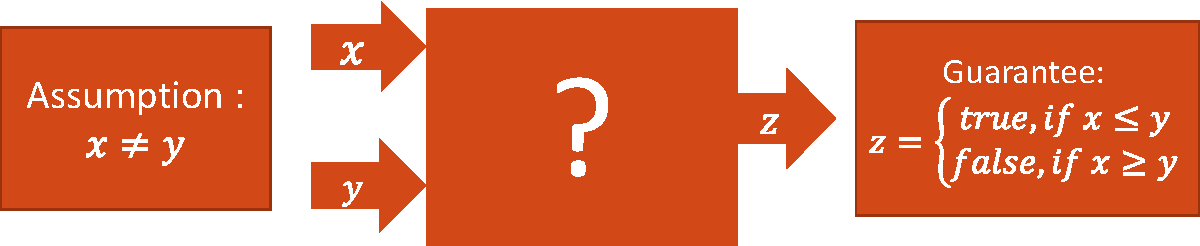
\includegraphics[width=\textwidth,height=\textheight,keepaspectratio]{real1-crop}    	
	\caption{Example of an Assume-Guarantee contract}
	\label{fg:example}
\end{figure}

As an illustrative example, consider the contract specified in
Figure~\ref{fg:example}. The component to be designed consists of two inputs,
$x$ and $y$ and one output $z$. If we restrict our example to the case of integer arithmetic,
we can see that the contract assumes that the inputs will never have the same value,
and requires that the output of the component is Boolean 
whose value depends on the comparison of the values of $x$ and $y$.
Also, notice that in the middle of the figure we depict the component using a
question mark symbol. The question mark simply expresses the fact that during
the early stages of software development, the implementation is absent or exists only partially.

Deciding existence of an implementation for the question-mark component 
that satisfies the specific contract for all possible inputs is aimed by the problem of 
\emph{realizability}, while automatically constructing a witness  of the proof 
of realizability of the contract is aimed by problem of \emph{program synthesis}.
The contract in Figure~\ref{fg:example} is obviously
\emph{realizable}, and therefore an implementation of the question-mark component exists.
Interestingly, if the assumption would be omitted then 
the contract is clearly \emph{unrealizable}, since no implementation 
is able to provide a correct output in the case where $x=y$.

\subsection{Formal Preliminaries}
\label{sec:pre}

For the purposes of this paper, we are describing a system using the types
$state$ and $inputs$. Formally, an \emph{implementation}, i.e. a
\emph{transition system} can be described using a set of initial states $I(s)$ of type $state \implies bool$, in addition to a transition relation $T(s,i,s')$ that
implements the contract and has type $state \implies inputs \implies
state \implies bool$.
 
An Assume-Guarantee contract can be formally defined by two sets, a set of
\emph{assumptions} and a set of \emph{guarantees}. The \emph{assumptions} $A$
impose constraints over the inputs, while the \emph{guarantees} $G$ are used for
the corresponding constraints over the outputs of the system and can be expressed as
two separate subsets $G_I$ and $G_T$, where $G_I$ defines the set of valid
initial states, and $G_T$ specifies the properties that need to be met during
each new transition between two states. Note that we do not necessarily expect
that a contract would be defined over all variables in the transition system,
but we do not make any distinction between internal state variables and outputs in the formalism.
This way, we can use state variables to, in some cases, simplify statements of guarantees.

\subsection{Realizability of Contracts}
The synthesis algorithm proposed in this paper is built on top of our realizability algorithm
originally presented in~\cite{Katis15:Realizability}. Using the formal foundations described in Sect.~\ref{sec:pre},
the problem of realizability is expressed using the notion of a state being \emph{extendable}:

\begin{definition}[One-step extension]
\label{def:extend}
A state $s$ is extendable after $n$ steps, denoted $\mathit{Extend}_{n}(s)$, if
any valid path of length $n-1$ starting from $s$ can be extended in response to
any input.%
%
\begin{multline*}%
\mathit{Extend}_{n}(s) \triangleq \forall i_1, s_1, \ldots, i_n, s_n.\\ A(s, i_1) \land G_T(s, i_1, s_1)
\land \cdots \land
A(s_{n-1}, i_n) \land G_T(s_{n-1}, i_n, s_n)
\implies \\
\forall i.~ A(s_n, i) \implies \exists s'.~ G_T(s_n, i, s')
\end{multline*}
\end{definition}

The algorithm for realizability uses Def.~\ref{def:extend} in two
separate checks that correspond to the two traditional cases exercised in
k-induction. For the $\mathit{BaseCheck}$, we ensure that all initial states are
extendable in terms of any path of length $k\le n$, while the inductive step of
$\mathit{ExtendCheck}$ tries to prove that all valid states are extendable.
Therefore, we attempt to find the smallest $n$, for which the two following 
$\forall\exists$-formulas are valid:%
%
\begin{equation}
\label{eq:sbcheck}
\mathit{BaseCheck}(n) \triangleq \forall k \leq n. (\forall s. G_I(s)
	  	\implies \mathit{Extend}_k(s))
\end{equation}%
%
\begin{equation}
\label{eq:echeck}
\mathit{ExtendCheck}(n) \triangleq \forall s. \mathit{Extend}_n(s)
\end{equation}

The realizability checking algorithm has been used to effectively find cases
where the traditional consistency check failed to detect conflicts between
stated requirements in case studies of different complexity and importance. It
has also been formally verified using the Coq proof assistant in terms of its
soundness, for the cases where it reports that a contract is realizable.

\subsection{Program Synthesis from Proofs of Realizability}

%While the implemented algorithm on realizability provided us with meaningful
%results during the verification of several contracts, 
The most important outcome of the work on realizability is that it 
 could be further used for solving a more complex problem of
\emph{program synthesis}, i.e., to automatically
derive implementations, given the same set of requirements as for the realizability checking.
Whenever a proof that a desired implementation for the given 
contract exists,  we can use this proof in order to construct a witness
implementation that satisfies the contract. 
%The limited power of SMT solvers
%in terms of solving formulas containing nested quantifiers immediately ruled
%out the prospect of using one as our primary synthesis tool. Fortunately, 
%we are able to exploit our prior results in the scope of solving validity and 
%Skolemizing $\forall\exists$-formulas (to be described in Sect.~\ref{sec:aeval}).

The idea behind our approach to solving the synthesis problem is
simple and elegant. Consider checks~\eqref{eq:sbcheck} and~\eqref{eq:echeck} that
are used in the realizability checking algorithm. Both checks require
that the reachable states explored are extendable using
Def.~\ref{def:extend}.
The key insight then is to decide if $\mathit{Extend}_{n}(s)$ is valid and generate a witness 
for each of the $n$ times that we run $\mathit{BaseCheck}$ and a final witness 
for the inductive case in $\mathit{ExtendCheck}$.

In the first order logic, witnesses for valid $\forall\exists$-formulas are represented by the Skolem functions.
Intuitively, a Skolem function expresses a connection between all universally quantified variables in the left-hand-side of the $\forall\exists$-formulas~\eqref{eq:sbcheck} and~\eqref{eq:echeck} and the existentially quantified variable $s'$ in the right-hand-side of the the formulas.
Our algorithm automatically generates such Skolem functions
while solving the validity of~\eqref{eq:sbcheck} and~\eqref{eq:echeck} and is described in details Sect.~\ref{sec:aeval}.

%GRIGORY: commented out the translation of A=> B => C into A /\ B => C since it is quite obvious

% Of course, 
%$\mathit{Extend}_{n}(s)$ as defined in~\eqref{def:extend} cannot
%be directly used for this purpose due to its form. This is not really an
%obstacle though, as we can rewrite the definition:
%
%\begin{multline*}
%\forall i_1, s_1, \ldots, i_n, s_n.\\ A(s, i_1) \land G_T(s, i_1, s_1)
%\land \cdots \land
%A(s_{n-1}, i_n) \land G_T(s_{n-1}, i_n, s_n)
%\implies \\
%\forall i.~ A(s_n, i) \implies \exists s'.~ G_T(s_n, i, s')
%\end{multline*}
%
%into an equivalent formula of the form $\forall \vec{x}.
%S(\vec{x}) \implies \exists \vec{y}. T(\vec{x},\vec{y})$ : 
%\begin{multline}
%	\label{ml:extendable2}
%		\forall i_1,s_1,\ldots,i_n,s_n,i. \\
%		A(s,i_1) \wedge G_T(s,i_1,s_1) \wedge \ldots \wedge
%		A(s_{n-1}, i_n) \wedge G_T(s_{n-1},i_n,s_n) \wedge A(s_n,i) \implies \\
%		\hspace{+2cm} \exists s'. G_T(s_n,i,s')
%	\end{multline}

%\begin{figure}
%\begin{small}
%\begin{verbatim}
%// for each variable in I or S,
%//   create an array of size k.
%//   then initialize initial state values
%assign_GI_witness_to_S;
%update_array_history;
%
%// Perform bounded 'base check' synthesis
%read_inputs;
%base_check'_1_solution;
%update_array_history;
%...
%read_inputs;
%base_check'_k_solution;
%update_array_history;
%
%// Perform recurrence from 'extends' check
%while(1) {
% read_inputs;
% \mathit{Extend}_check_k_solution;
% update_array_history;
%}
%\end{verbatim}
%\end{small}
%\caption{Algorithm skeleton for synthesis}
%\label{fig:algorithm}
%\end{figure}

\begin{algorithm2e}[tb!]
\SetAlgoSkip{}
\SetKwFor{While}{forever}{do}{}
\KwIn{\grigory{tbd}}

\BlankLine
  \textsc{assign\_GI\_witness\_to\_S()}; 	\Comment{Initialize  state values in an array of size $k$.}\\
  \textsc{update\_array\_history()}\;

\BlankLine
  \textsc{read\_inputs()}; 		\Comment{Perform bounded ``base check'' synthesis}\\
  \textsc{base\_check\_1\_solution()}\;
  \textsc{update\_array\_history()}\;
  $\ldots$\\
  \textsc{read\_inputs()}\;
  \textsc{base\_check\_k\_solution()}\;
  \textsc{update\_array\_history()}\;
  
\BlankLine  

\While{}{  
 \textsc{read\_inputs()}; 		\Comment{Perform recurrence from ``extends'' check}\\
 \textsc{extend\_check\_k\_solution()}\;
 \textsc{update\_array\_history()}\;
}

\caption{Synthesized implementation.}
\label{alg:synt}
\end{algorithm2e}

\grigory{The algorithm description should be improved. Currently it mixes both, the synthesized implementation, and the synthesis procedure itself. There is an infinite loop that clearly belongs to the implementation, but the reviewers may misunderstand it. Of course, we should explicitly point that the synthesis procedure always terminates since there is a need to solve and skolemize finite number of formulas.}

Thus, we can construct the skeleton of an algorithm as shown in Alg.~\ref{alg:synt}.  
The algorithm stars (method \textsc{assign\_GI\_witness\_to\_S()}) with creating an array for each input and history variable up to depth
$k$, where $k$ is the depth at which we found a solution to our realizability algorithm.
In each array, the zeroth element is the ``current'' value of the variable, the first element is the previous value, and the $(k-1)$'th value is the $(k-1)$-step previous value.

The algorithm then generates witnesses for each of the $\mathit{BaseCheck}$ instances of
successive depth to describe the initial behavior of
the implementation up to depth $k$.  This process starts from the memory-free
description of the initial state ($G_I$). 
There are two ``helper'' operations:
\textsc{update\_array\_history()} shifts each element in the arrays one position forward
(the $(k-1)$'th value is simply forgotten), and \textsc{read\_inputs()} reads the current values of inputs into the zeroth element of the input variable arrays.  Once the history is entirely initialized using the $\mathit{BaseCheck}$ witness values, 
the algorithm generates a witness for the $\mathit{ExtendCheck}$ instance to describe the recurrent behavior of
the implementation, i.e., the next value of outputs in each iteration in the infinite loop.

 \andreas{Add proof of correctness here}
 
 \subsection{Running Example}
 
 To further understand the concepts described in this paper, we provide a simple
 running example that is representative of what happens internally during a
 single run of the synthesis algorithm. Figure~\ref{fg:example} is showing a
 simple automaton that we will be using as the example. To the right, we can see
 the requirements that were written for the automaton in the Lustre language.
 The specification mentions one input, namely $x$. While the $state$ variable
 would otherwise be considered as the output in the resulting implementation,
 we use a simple hack that prevents us from explicitly defining how it should
 be assigned, by adding it as an actual input to the specification. In addition
 to the previous, can see that there are 4 properties to be checked, along with a
 JKind-specific query on the specification's realizability. Properties
 \textit{prop2} and \textit{prop3} are used to indirectly summarize parts of the
 possible transitions in the automaton. Properties \textit{prop1} and
 \textit{prop4} are requirements with respect to two local variables, \textit{bias}
 and \textit{bias\char`_max}. Variable \textit{bias} calculates the number of successive
 ones or zeros read by the automaton, while \textit{bias\char`_max} is used as a flag
 to indicate that at least two zeros or two ones have been read in a row.
 
\begin{figure}[H]
\begin{minipage}[c]{0.35\textwidth}
\centering
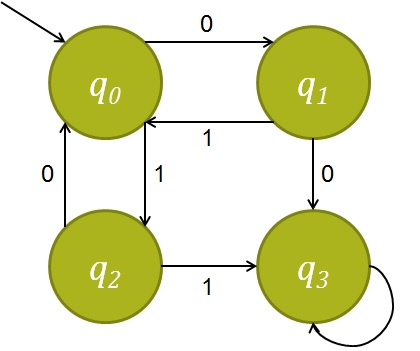
\includegraphics[width=\textwidth,height=\textheight,keepaspectratio]{example}
\end{minipage}
\begin{minipage}[c]{0.7\textwidth}
 \begin{Verbatim}[fontsize=\scriptsize]
node top(x : bool; state: int) returns (  );
var
  bias : int;
  prop1, prop2, prop3, prop4, prop_all : bool;
  bias_max : bool;
let

  bias = 0 -> (if x then 1 else -1) + pre(bias);
  bias_max = false ->
	(bias >= 2 or bias <= -2) or pre(bias_max);
  prop1 = (state = 0 => (bias = 0));
  prop2 = true ->
  	(pre(state = 0) and x) => state = 2;
  prop3 = true ->
  	(pre(state = 0) and not x) => state = 1;
  prop4 = bias_max => state = 3;
  prop_all = prop1 and prop2 and prop3 and prop4;
  --%PROPERTY prop_all;
  --%REALIZABLE x;
tel;
 \end{Verbatim}
\end{minipage}
\caption{Automaton and Requirements for running example}
\label{fg:example}
\end{figure}

Considering these requirements, we want an answer to whether this model is
realizable. We provide the model as an input to JKind, and observe the results.
The model is sufficiently simple to be declared as realizable by the tool, and
thus can be further examined in terms of synthesizing a representative
implementation. Using the k-inductive proof of realizability, which happens to
be of length $k = 1$, we forward the two $\forall\exists$-formulas (one for the
base check, and one for the inductive check) to be skolemized by AE-VAL. From
this process, we receive two Skolem functions, that effectively describe
possible assignments to the local variables of the specification, as well as the
output \textit{state} (we can effectively decide what is an output by excluding
it from the list of arguments in the \textit{--\%REALIZABLE} query above). We
can then use these two Skolem functions to construct the final implementation
following the outline provided in Alg.~\ref{alg:synt}. Due to the fact that the
implementation is too long to be included here (135 Lines of Code), we do not
present its actual form. The main idea involves the redefinition of each
variable in the model as an array of size equal to the proof's length $k$, and,
using the $k$-th element of each array as the corresponding output of the call
to $k$-th Skolem function. After this initialization process, we use an infinite
loop to assign new values to the element corresponding to the last Skolem
function, to cover the inductive step of the original proof. One of the
interesting features that come from using a k-inductive proof is that we can
possible refer to up to $k-1$ values of each variable in the past, and as such
an update process occurs in between each iteration of the infinite loop, to only
keep the latest k values assigned to each element of each array.
